\chapter[Background]{Background\footnote{Includes text and images from minor thesis 'Business ideation for \gls{ble}'}}

\section{Overview of \acrlong{ble}}
Rest of overview, from what is missed in 1st chapter.

\subsection{Design objectives of \gls{ble}}
\gls{ble} was designed by Bluetooth \gls{sig} from the ground up, which helped it achieve certain design goals. These design goals for this wireless personal area network were \emph{low cost, worldwide operation, short range, robustness} and \emph{low power}\cite{Heydon2012}. 
\paragraph{Low Power} \gls{ble} aims to use a tiny batteries such as button cell to keep a device operating for months to years. To achieve this goal, \gls{ble} was optimized to communicate small amounts of data, such as the states of devices. Also \gls{ble} is optimized to have lower peak power requirements, which allows use of button cells to be used with \gls{ble} devices.
\paragraph{Worldwide Operation}
For a technology to be adopted, it is important that there is uniform conformity to the regulations around the world. The 2.4 \si{\GHz} \gls{ism} radio band is the only one available license free worldwide. The technology to develop wireless devices in this band is mature making it the suitable radio band for \gls{ble}.
\paragraph{Short Range}
\gls{ble} was designed to be for personal area network like Classic Bluetooth, which means that it is not a network to work with a cellular base station network. This design criterion goes hand in hand with \emph{low power}.
\paragraph{Low Cost} Lower power requirements mean that the batteries in \gls{ble} devices need to smaller and have to be replaced less frequently, both resulting in a reduction of cost for both the manufacturer and the customer. The use of the \gls{ism} band for communication levels removes the licensing entry barrier for start-ups to develop \gls{ble} devices. \gls{ble} embraces simplicity in its pursuit to lower the cost. \gls{ble} supports only single-hop communication in a star network, which reduces the memory and processor requirement for supporting the protocol. Simplicity was the key factor for the choosing of \gls{gfsk} as the modulation scheme for \gls{ble} to result in low cost, small radio implementation of the radio in the \glspl{ic} for \gls{ble}. 
\paragraph{Robustness} The 2.4~\si{\GHz} space is crowded with devices communicating with various standards as well as spurious noise making the robustness a key criteria in developing \gls{ble} standard. \gls{ble} uses a multi-channel hopping mechanism called \gls{afh} to detect, avoid and recover from interference. In addition to \gls{afh}, \gls{ble} uses \gls{crc} to detect and recover from bit-errors due to background noise.

\subsection{\gls{ble} network architecture}
Single and Dual devices,
Advertisers and scanners,
Master and Slave,
Star Network,
figure \ref{devicesBLE}
\begin{figure}[h] %{r}{0.51\textwidth}
%\vspace{-15pt}
  \begin{center}
	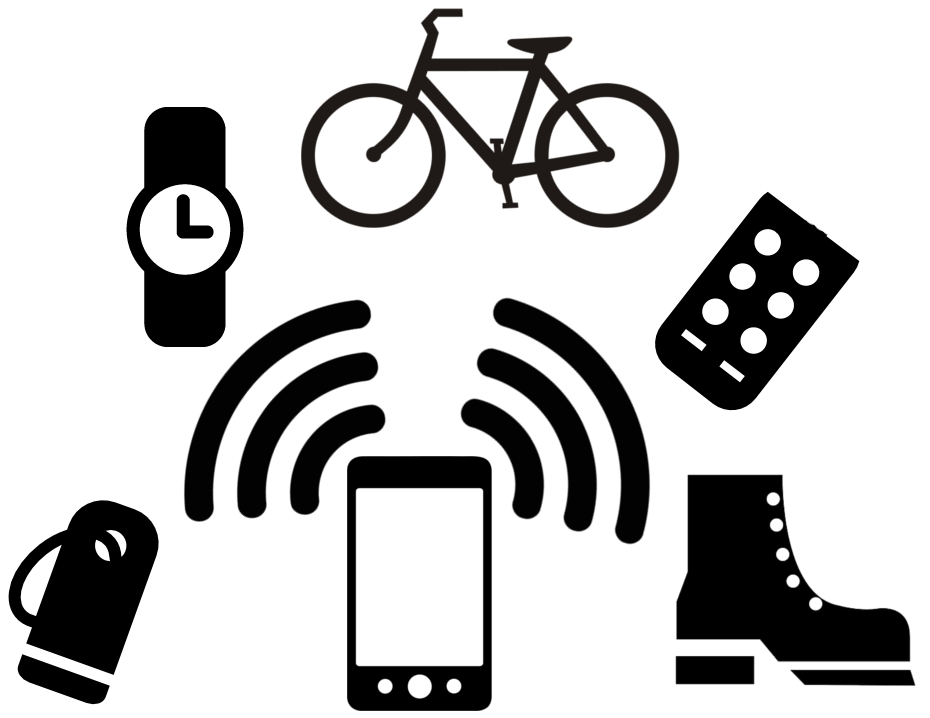
\includegraphics[width=0.49\textwidth]{devicesBLE}
  \end{center}
\caption{Typical BLE network}
%\vspace{-10pt}
\label{devicesBLE}
\end{figure}

\section{\gls{ble} stack overview}
Explain host and controller division. More details about link layer.

\textbf{Image of the stack}

The link layer of 802.15.4 consists of \gls{mac} layer on top of a \gls{rdc} layer. For the RDC layer the Null-RDC and ContikiMAC driver will be tested in each of the test with \gls{csma} as the \gls{mac} layer. In case of Contiki-MAC the receiving node switches on periodically to sense if there are any packets that need to be received. The default time of this period is 125 ms. In case of null-RDC the radio receiver is never switched off, as the name suggests.

In \gls{ble}, the devices can assume different roles in the different layers of the protocol. In the link layer a device can be a 'Master' or a 'Slave'. In the \gls{att} layer, a device can be a 'Client' and/or 'Server'. A server contains data and the client can request data from the server.

\paragraph{Physical layer}
\paragraph{Link layer}
\paragraph{\gls{l2cap}}
\paragraph{\gls{gap}}
\paragraph{\gls{att}}
\paragraph{\gls{gatt}}
\paragraph{\gls{sm}}

\section{Overview of Contiki}
??????????????? Which aspects of Contiki here?

\section{Overview of 802.15.4}
Mention that in this thesis the Contiki specific implementations of the 802.15.4 layers will be tested.

\subsection{Physical layer}

\subsection{\gls{mac} layer}
\subsubsection{\gls{rdc} layer}
\subsubsection{\gls{csma}}


